%start preamble
\documentclass[paper=a4,fontsize=11pt]{scrartcl}%kind of doc, font size, paper size

\usepackage{fontspec}
\defaultfontfeatures{Ligatures=TeX}
%\setsansfont{Liberation Sans}
\usepackage{polyglossia}	
\setdefaultlanguage[spelling=new, babelshorthands=true]{german}
\usepackage{csquotes}
		
\usepackage{amsmath}%get math done
\usepackage{amsthm}%get theorems and proofs done
\usepackage{graphicx}%get pictures & graphics done
\graphicspath{{pictures/}}%folder to stash all kind of pictures etc
\usepackage{hyperref}%for links to web
\usepackage{amssymb}%symbolics for math
\usepackage{amsfonts}%extra fonts
\usepackage []{natbib}%citation style
\usepackage{caption}%captions under everything
\usepackage{listings}
\usepackage[titletoc]{appendix}
\numberwithin{equation}{section} 
\usepackage[printonlyused,withpage]{acronym}%how to handle acronyms
\usepackage{float}%for garphics and how to let them floating around in the doc
\usepackage{cclicenses}%license!
\usepackage{xcolor}%nicer colors, here used for links
\usepackage{wrapfig}%making graphics floated by text and not done by minipage
\usepackage{dsfont}
\usepackage{stmaryrd}
\usepackage{geometry}
\usepackage{fancyhdr}
\usepackage{menukeys}
\usepackage{enumitem}



%settings colors for links
\hypersetup{
    colorlinks,
    linkcolor={blue!50!black},
    citecolor={blue},
    urlcolor={blue!80!black}
}

\definecolor{pblue}{rgb}{0.13,0.13,1}
\definecolor{pgreen}{rgb}{0,0.5,0}
\definecolor{pred}{rgb}{0.9,0,0}
\definecolor{pgrey}{rgb}{0.46,0.45,0.48}

\pagestyle{fancy}
\lhead{Netzwerke und verteilte Systeme\\
 Übung\\ Wintersemester 2021/22}
\rhead{FB-4\\Informatik in Kultur und Gesundheit\\ HTW-Berlin}
\lfoot{Virtualisierung mit VirtualBox}
\cfoot{}
\fancyfoot[R]{\thepage}
\renewcommand{\headrulewidth}{0.4pt}
%\renewcommand{\footrulewidth}{0.4pt}

\lstdefinestyle{Bash}{
  language=bash,
  showstringspaces=false,
  basicstyle=\small\sffamily,
  numbers=left,
  numberstyle=\tiny,
  numbersep=5pt,
  frame=trlb,
  columns=fullflexible,
  backgroundcolor=\color{gray!20},
  linewidth=0.9\linewidth,
  %xleftmargin=0.5\linewidth
  upquote=true,
  columns=fullflexible,
  literate={*}{{\char42}}1
         {-}{{\char45}}1
}


%%here begins the actual document%%
\newcommand{\horrule}[1]{\rule{\linewidth}{#1}} % Create horizontal rule command with 1 argument of height


\DeclareMathOperator{\id}{id}

\title{	
\normalfont \normalsize 
\textsc{Übungsblatt 01 -- Shell Grundlagen}
}
\begin{document}
\begin{center}
\Large{\textbf{Übungsblatt 1 -- Shell Grundlagen}}
\end{center}
Diese Übung soll sie zunächst mit dem Umgang unixoider Betriebssysteme vertraut machen, sodass der Einstieg etwas leichter fällt. Im speziellen ist hier der Umgang mit der Kommandozeile gemeint, da Server-Systeme i.A. keine grafische Schnittstelle anbieten.\\
Die Erfahrung zeigt, dass einige Studierende zunächst überfordert sind. Keine Sorge: Sie sind nicht allein.\\
Generell hilft es am Ball zu bleiben und sich kontinuierlich mit den Aufgaben zu beschäftigen -- das heißt auch: selber recherchieren, Literatur lesen, sich Unklarheiten bewusst machen und entsprechende Fragen stellen.

\begin{center}\Large{\textbf{Aufgabe A -- Shell Basics}}\end{center}\vskip0.25in
%\setlist[enumerate, 1]{itemsep=\baselineskip}
\begin{enumerate}
\item Navigation:\\
Ziel dieser Aufgabe ist die grundlegende Navigation in der Shell zu verstehen.
\begin{enumerate}[label=(\alph*)]
		\item Starten sie die VM! Sie können sich als Nutzer \emph{student} mit dem Passwort \emph{student} anmelden. (Ja, das Passwort ist beim eintippen nicht zu sehen!)
		\begin{figure}[h]
		\centering
		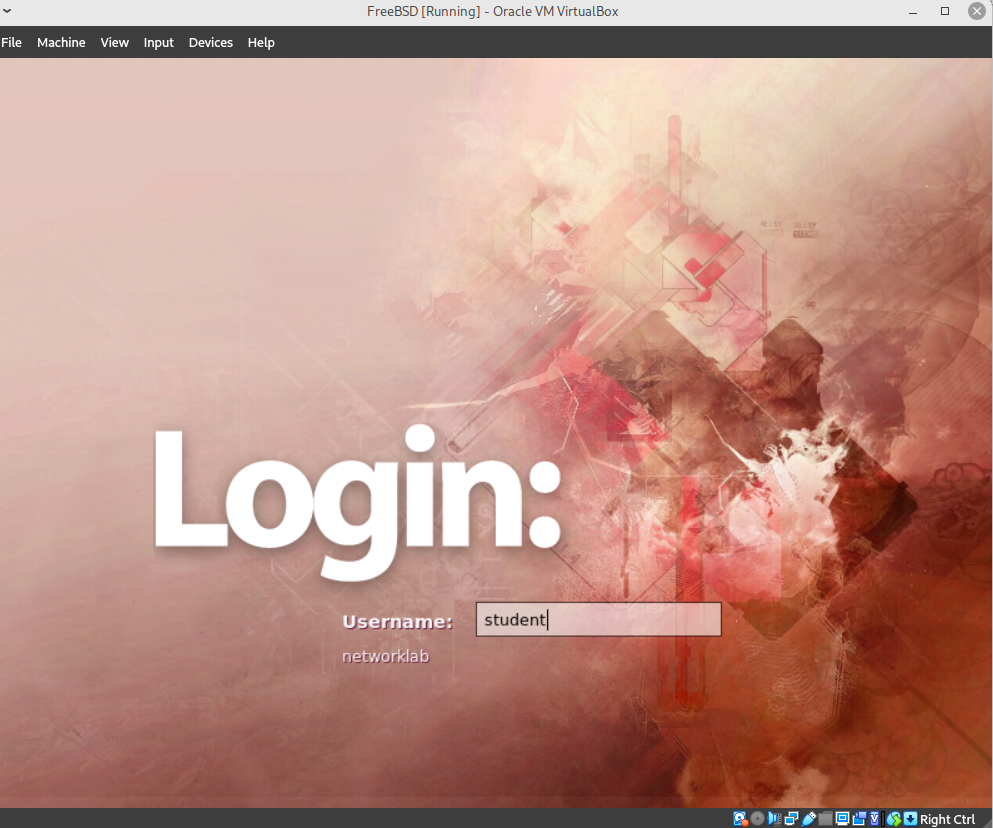
\includegraphics[scale=0.3]{freebsd_login}
		\end{figure}
		\item Mit dem Befehl \emph{startx} können sie die grafische Oberfläche starten -- müssen es aber nicht. Sie sind im Betriebssystem angemeldet und können alle Aufgabe lösen.\\
		Falls sie unter der GUI arbeiten: Starten sie die Kommandozeile (Shell)! Entweder via Tastenkombination \keys{\ctrl + \Alt + t} (STRG + ALT + T) oder über das Menü bzw. das Icon im Panel.\\
		Lassen sie sich anschließend Ihr aktuelles Verzeichnis auf der Kommandozeile ausgeben! Dies ist standardmäßig ihr Heimatverzeichnis \footnote{Auch \enquote{home directory}: $\sim$ oder ausgeschrieben \path{/home/student/} auf der VM bzw. \path{/home/s0xxxxxx} auf den Laborrechnern}.
		\item Lassen sie sich den Inhalt des Verzeichnisses ausgeben.
		\item Navigieren sie via \emph{cd} in den Ordner \path{/var}
		\item Springen sie vom vorherigen Ordner in den übergeordneten Ordner (\emph{/} -- root).
		\item Navigieren sie in Ihr Heimatverzeichnis (Dies sollte durch genau ein Kommando erfolgen!)
		\item Recherchieren sie kurz den Unterschied zwischen relativen und absoluten Pfaden in Unix-Dateisystemen. Sie können folgende Quelle hierfür nutzen: \url{https://de.wikipedia.org/wiki/Pfadname}
		\item Lassen sie sich mit dem Befehl \emph{history} die letzten Befehle Anzeigen, die im Terminal ausgeführt wurden. 
		\item Benutzen sie die Pfeiltasten \keys{\arrowkeyup} und \keys{\arrowkeydown}, um die letzten Befehle auf die Kommandozeile zu bringen. Mithilfe der Pfeiltasten können sie durch die Historie der bereits genutzten Befehle navigieren, wobei \keys{\arrowkeyup} in Richtung älterer Befehle und \keys{\arrowkeydown} Richtung neuerer springt.
		\item Mit der Tastenkombination \keys{\ctrl +r} öffnen Sie die interaktive Suche der History anstoßen. Unter Ihrem Command-Prompt erscheint folgendes:\\
		\begin{lstlisting}[style=Bash, language=Bash]
bck-i-search: _
		\end{lstlisting}
		Mithilfe dieser Suche können sie nach bereits benutzten Befehlen suchen. Wenn sie beispielsweise \emph{cd} eingeben sehen Sie den zuletzt genutzten Befehl der den Token \emph{cd} enthält. Durch wiederholtes Drücken der Tastenkombination \keys{\ctrl +r} durchsuchen Sie die History Richtung älterer Befehle die das angegebene Schlüsselwort enthalten.\\
		\textbf{Kommandos:} \textcolor{blue}{\emph{cd}, \emph{cd ..}, \emph{cd \textasciitilde} \emph{pwd}, \emph{history}}
	\end{enumerate}
	\item Grundlegende Kommandos:\\
  Um den grundlegenden Umgang mit der Shell kennenzulernen fertigen Sie sich ein eigenes kleines Shell-Tutorial an.\\
  \textbf{Hinweis:} Um lästige Tipparbeit zu vermeiden, bieten viele Shells eine Autovervollständigung an. Mit der \keys{\tab}-Taste (Tabulatortaste) kann diese genutzt werden -- sie müssen lediglich die ersten Buchstaben tippen und können durch (mehrmaliges) drücken der Tabulatortaste den begonnenen Befehl vervollständigen. Wenn es mehrere Alternativen der Vervollständigung gibt, kann zwischen diesen gesprungen werden.\\
  Schauen sie in die Aufgabe B, wenn bestimmte Kommandos (noch) nicht wie gewünscht arbeiten! Ein Blick in die Hilfe löst dies in vielen Fällen.
  	\begin{enumerate}[label=(\alph*)]
  		\item Erzeugen sie das Verzeichnis \path{shell_tutorial} und wechseln sie in das erzeugte Verzeichnis. Erzeugen sie darin eine leere Datei mit dem Dateinamen \textit{shell\_tutorial.md}.\footnote{.md steht für Markdown, welches ein Format für Textdateien ist, ähnlich wie .txt oder .doc-Dateien.} (\textbf{Der Satzpunkt gehört nicht zum Dateinamen!})\\
        \textbf{Achtung:} Verwenden sie zum Anlegen der Datei keinen Editor, sondern (einen) Kommandozeilenbefehl(e).\\
        \textbf{Kommandos:} \textcolor{blue}{\emph{touch}, \emph{mkdir}, \emph{cd}}
		\item Überprüfen sie die Dateigröße der Datei \textit{shell\_tutorial.md}.\\
		\textbf{Kommandos:} \textcolor{blue}{\emph{ls}, \emph{stat}, \emph{du}}
		\item Fügen sie mithilfe der Umleitung der Standardausgabe die Zeilen "Shell Tutorial", sowie eine (neue) Zeile mit dem aktuellen Datum ein.\\
		\textbf{Kommandos:} \textcolor{blue}{\emph{echo}, \emph{date}, $>>$, bzw. \emph{>}}
		\begin{itemize}
			\item \small Verwenden sie für das Einfügen des Textes keinen Editor, sondern einen Befehl und eine Weiterleitung (Umleitung der Standardausgabe).
		\end{itemize}
		\item Geben sie die erste Zeile der Datei auf der Kommandozeile aus.\\
		\textbf{Kommandos:} \textcolor{blue}{\emph{head}, \emph{tail}, \emph{more}, \emph{less}}
		\item Öffnen sie Ihr Cheat-Sheet mithilfe das Programms \emph{vim}, \emph{emacs} oder via \emph{retext}. Notieren sie sich alle Befehle, sowie deren Bedeutung, sodass sie eine erste Anlaufstelle für die nächsten Übungen haben. Dieses Dokument (Sie können auch mehrere anlegen) sollten sie fortan als Notizzettel für die Laboraufgaben nutzen!
		\item Navigieren sie in Ihr Heimatverzeichnis. Legen sie folgenden Ordner, sowie Unterordner mithilfe des \emph{mkdir}-Kommandos an: \path{exercise_notes/tutorials}. (Satzpunkt gehört wieder nicht zum Dateinamen!)
		\item Kopieren sie die Datei bzw. den Ordner \emph{shell\_tutorial} in das eben angelegte Verzeichnis.\\
		\textbf{Kommandos:} \textcolor{blue}{\emph{cp} }
        \item Kopieren sie die Datei(en) inklusive des Ordners \path{exercises/tutorials/shell_tutorial.md} in das Verzeichnis \path{/tmp}.\\
        \textbf{Hinweise:} Schauen sie in die Manpage von \emph{cp} um herauszufinden, wie Ordner kopiert werden können.\\
        \textbf{Kommandos:} \textcolor{blue}{\emph{man cp}}
  	\end{enumerate}
  	\footnote{.md steht für Markdown, welches ein Format für Textdateien ist, ähnlich wie .pdf oder .doc-Dateien.}
\newpage        
         \item Benutzer- \& Systeminfos:
    		\begin{enumerate} [label=(\alph*)]
          \item Lassen sie sich den Nutzernamen und die Gruppenzugehörigkeit auf dem Terminal des Rechners ausgeben.\\
          \textbf{Kommandos:} \textcolor{blue}{\emph{id}, \emph{groups}, \emph{whoami}}
          \item Lassen sie sich den Namen ihrer VM ausgeben.\\
          \textbf{Kommandos:} \textcolor{blue}{\emph{hostname}}
          \item Legen sie einen Ordner \emph{.nfo} an. Schreiben Sie die Ausgaben Ihres Nutzernamens, Gruppenzugehörigkeit sowie den Namen des genutzten Rechners in die Datei \emph{info.nfo} in den Ordner \emph{.nfo}.
          \item Nutzen sie \emph{ls} und prüfen sie, ob sie den Ordner wiederfinden können! Finden sie heraus, wie sie mithilfe des \emph{ls} Kommandos trotzdem diesen versteckten Ordner (Hidden-Folder) finden können.
          \item Löschen sie erst die \emph{nfo}-Datei. Anschließend den Ordner \emph{.nfo}\\
          \textbf{Kommandos:} \textcolor{blue}{\emph{rm}}
          \item Bringen sie das genutzte Betriebssystem, sowie dessen Kernel in Erfahrung.\\
          \textbf{Kommandos:} \textcolor{blue}{\emph{freebsd-version}, \emph{uname}}
        \end{enumerate}
        \item Sudo/Doas -- Recherchieren sie, wie und was der Befehl \emph{sudo/doas} leisten kann.\\
        Eine Anlaufstelle wäre: \url{https://www.freebsd.org/doc/de_DE.ISO8859-1/books/handbook/security-sudo.html}
\end{enumerate}

\begin{center}\Large{\textbf{Aufgabe B -- Manpages \& Hilfe}}\end{center}\vskip0.25in
Unix bietet von Hause aus einige Anlaufstellen an, mit deren Hilfe sie die Handhabung von der Tools (Kommandozeilenbefehle etc.) recherchieren können.
\begin{enumerate}
	\item Suchen sie sich einen Befehl aus den sie heute bereits benutzt haben. Mithilfe der Parameter \emph{--help}, \emph{-help} oder \emph{-h} erhalten Sie eine kurze Übersicht über den Befehl.
    \item Rufen sie die \emph{manpage} für einen beliebigen Befehl ein: \\
    		\emph{man HIERBEFEHLKEINFUEGEN}\\
		 Nutzen sie die Pfeiltasten, die Bild hoch/runter (\keys{pageup \arrowkeyup}/ \keys{pageup \arrowkeydown}) oder Leertaste (\keys{\Space}) zum lesen. Schließen erfolgt mit \keys{q}. Mit \emph{/} könne sie innerhalb der Manpage suchen.
\end{enumerate}
Die Manpages finden sie als Website auch im Internet. \footnote{\url{https://linux.die.net/man/}}

\begin{center}\Large{\textbf{Aufgabe C -- User \& Rechte}}\end{center}\vskip0.25in
%\setlist[enumerate, 1]{itemsep=\baselineskip}
\begin{enumerate}
\item Diskrete Zugangskontrolle (DAC) -- Nutzer \& Gruppen
	\begin{enumerate}[label=(\alph*)]
        \item Recherchieren sie die Bedeutung der Spalten 1 -- 7 der Ausgabe des Kommandos \emph{ls -la} in ihrem Heimatverzeichnis.
        \item Finden sie die Datei bzw. das Programm \textit{reboot}, die den Neustart des Systems veranlassen kann. Lassen Sie sich die Rechte der Datei \textit{reboot} ausgeben!
        \textbf{Kommandos:} \textcolor{blue}{\emph{whereis}, \emph{find}}
        \item Um was für einen Dateitypen handelt es sich hierbei? Was ist reboot für eine Datei -- recherchieren Sie gegebenenfalls kurz.
        \item Wer ist der Eigentümer, wie sehen die Berechtigungen für Nutzer, Gruppe und Andere in symbolischer, oktaler und binärer Schreibweise aus?
        \item Führen sie einen Reboot des Systems durch -- Achtung speichern sie alle offenen Dateien, nicht gesepeicherte Inhalte gehen sonst verloren!
  \end{enumerate}
\end{enumerate}
\begin{center}\Large{\textbf{vi/vim}}\end{center}\vskip0.25in
\begin{enumerate}
	\item Der Standardeditor unter Unix ist \emph{vi}, dieser ist auf jedem System vorhanden. Bearbeiten sie folgendes Tutorial:\\
	\url{http://www.openvim.com/}\\
	Ein Cheat-Sheet kann unter:\\
	\url{https://www.fprintf.net/vimCheatSheet.html}\\
	bezogen werden, sodass die Nutzung etwas leichter fällt.\\
	Sie müssen kein vi-Guru werden, jedoch sollten sie wissen, wie Dateien geöffnet, geschlossen, gespeichert werden, sowie wie im vi/vim navigiert wird und wie Sie den \emph{vi} verlassen können. Notieren sie sich in ihrem Cheat-Sheet wie sie vorgegangen sind!\\
	Die Navigation in den Manpages entspricht der des vi/vims.
	\item Nutzen sie den \emph{vi(m)}-Editor, um den Hostnamen der virtuellen Maschine zu ändern. Sie können einen beliebigen Namen wählen, es empfiehlt sich einen Namen zu wählen, der die Funktionalität widerspiegelt.
\end{enumerate}

\begin{center}\Large{\textbf{Reboot \& Poweroff}}\end{center}\vskip0.25in
\begin{enumerate}
	\item Sie können das System mit dem Befehlt \emph{sudo reboot} neu starten.
	\item Mithilfe des Befehls \emph{poweroff} können sie das System herunterfahren.
\end{enumerate}

Weiter geht es mit dem zweiten Übungsblatt: Netzwerkinfrastruktur 1!

\end{document}